\documentclass[10pt]{beamer}
\usepackage{amsmath,amssymb,longtable,hhline}
\usepackage{mathrsfs}
\usepackage{xcolor}
\usepackage{hyperref}
\usepackage{multicol}
\usepackage{anyfontsize}
\usepackage{minted}
\usepackage{alltt}

\usemintedstyle{tango}
\newcommand{\ltprgsize}{\fontsize{5}{5}\selectfont}
%\newcommand{\ltprgsize}{\footnotesize}
\setminted{fontsize=\footnotesize,mathescape}

\definecolor{mygreen}{rgb}{0,0.6,0}
\definecolor{mygray}{rgb}{0.5,0.5,0.5}
\definecolor{mymauve}{rgb}{0.58,0,0.82}

\hypersetup{
    bookmarks=true,         % show bookmarks bar?
    unicode=true,           % non-Latin characters in Acrobat’s bookmarks
    pdftoolbar=false,        % show Acrobat’s toolbar?
    pdfmenubar=false,        % show Acrobat’s menu?
    pdffitwindow=false,     % window fit to page when opened
    pdfstartview={FitH},    % fits the width of the page to the window
    pdftitle={},    % title
    pdfauthor={Evgeny Cherkashin},     % author
    pdfsubject={model driven architecture},   % subject of the document
    pdfnewwindow=true,      % links in new PDF window
    colorlinks=true,       % false: boxed links; true: colored links
    linkcolor=red,          % color of internal links (change box color with linkbordercolor)
    citecolor=green,        % color of links to bibliography
    filecolor=magenta,      % color of file links
    urlcolor=blue           % color of external links
}

\usepackage{pifont}

\usetheme{Warsaw}
\usecolortheme{crane}
%\useinnertheme{rectangles}
%\setbeamertemplate{itemize item}{\scriptsize\hbox{\donotcoloroutermaths\ding{113}}}
\definecolor{darkding}{RGB}{200,56,0}
\setbeamertemplate{itemize item}{\scriptsize\hbox{\color{darkding}{\bfseries\ding{113}}}}
\setbeamertemplate{itemize subitem}{\tiny\raise1.5pt\hbox{\donotcoloroutermaths$\blacktriangleright$}}
\setbeamertemplate{itemize subsubitem}{\tiny\raise1.5pt\hbox{\donotcoloroutermaths$\blacktriangleright$}}
\setbeamertemplate{enumerate item}{\insertenumlabel.}
\setbeamertemplate{enumerate subitem}{\insertenumlabel.\insertsubenumlabel}
\setbeamertemplate{enumerate subsubitem}{\insertenumlabel.\insertsubenumlabel.\insertsubsubenumlabel}
\setbeamertemplate{enumerate mini template}{\insertenumlabel}

\beamertemplatenavigationsymbolsempty

\usepackage{iftex,ifxetex}
\ifPDFTeX
  \usepackag
%\useoutertheme{split}
%\useinnertheme{rounded}
\setbeamertemplate{background canvas}[vertical shading][bottom=white!80!cyan!20,top=cyan!10]
%\setbeamertemplate{sidebar canvas left}[horizontal shading][left=white!40!black,right=black]

\graphicspath{{pics/}}

\providecommand{\email}[1]{\texttt{#1}}
\usepackage{changepage}
\newcommand{\GB}[1]{\colorbox{green}{#1}}
\newcommand{\BB}[1]{\colorbox{blue}{#1}}
\newcommand{\RB}[1]{\colorbox{red}{#1}}
\newcommand{\btprgsize}{\fontsize{7}{7}\selectfont}

% --------------------------

\begin{document}

\Setbeamertemplatee[utf8]{inputenc}
  \usepackage[T1]{fontenc}
  \usepackage[russian]{babel}
  \usepackage{lmodern}
  \usefonttheme{serif}
\else
  \ifluatex
    \usepackage{unicode-math}
    \defaultfontfeatures{Ligatures=TeX,Numbers=OldStyle}
    \setmathfont{Latin Modern Math}
    \setsansfont{Linux Biolinum O}
    \setmonofont{Fira Mono}[Scale=MatchLowercase]
    \usefonttheme{professionalfonts}
    % \setmathfont[
    %     Ligatures=TeX,
    %     Scale=MatchLowercase,
    %     math-style=upright,
    %     vargreek-shape=unicode
    %     ]{euler.otf}
  \fi
\fi

%\useoutertheme{split}
%\useinnertheme{rounded}
\setbeamertemplate{background canvas}[vertical shading][bottom=white!80!cyan!20,top=cyan!10]
%\setbeamertemplate{sidebar canvas left}[horizontal shading][left=white!40!black,right=black]

\graphicspath{{pics/}}

\providecommand{\email}[1]{\texttt{#1}}
\usepackage{changepage}
\newcommand{\GB}[1]{\colorbox{green}{#1}}
\newcommand{\BB}[1]{\colorbox{blue}{#1}}
\newcommand{\RB}[1]{\colorbox{red}{#1}}
\newcommand{\btprgsize}{\fontsize{7}{7}\selectfont}

% --------------------------

\begin{document}

\setbeamertemplate{background canvas}[vertical shading][bottom=white,top=white]
\setbeamercolor{background canvas}{bg=white}

\title{Technologies of Semantic WEB as an environment of application development and integration}
\author[E.~Cherkashin]{\bfseries%
  Evgeny Cherkashin, Nikita Dorodnykh, Alexey Shigarov, \emph{et al.}}
\institute{\normalsize Matrosov Institute for System Dynamics and Control Theory of Siberian Branch of Russian Academy of Sciences, Irkutsk, Russia\\%
  \email{\href{mailto:eugeneai@icc.ru}{eugeneai@icc.ru}}%
}
\date[2021]{AICTS'2021, December, 06, 2021 \\
Irkutsk, Russia}
%\date{\today}
\maketitle

\begin{frame}
\frametitle{Research and Development objectives}
\textbf{Main objective} of the activity is to construct data integration tools based on the \textbf{standardized} Semantic WEB technologies.

The following aspects are under consideration:
  \begin{enumerate}
  \item Application data representation
  \item Ontological model representation
  \item Document publication
  \item Application integration % via knowledge graph data documents
  \item Model transformation
  \end{enumerate}
\end{frame}

\begin{frame}
\frametitle{Representation of ontological models}
The ontologies are represented with \texttt{<subject,~predicate,~object>} \textbf{triples} as \textbf{graphs}, and there is frequently a \textbf{context}, the graph itself.
\begin{columns}
  \begin{column}{0.5\linewidth}
    \includegraphics[width=\linewidth]{SPO.pdf}
    \mbox{}\\[1em]
    \includegraphics[width=\linewidth]{socrates-human.pdf}
  \end{column}
  \begin{column}{0.5\linewidth}
    % Graph comprises
    % \begin{itemize}
    % \item T-Box
    % \item {\color{blue}{A-Box}}
    % \end{itemize}
    The subjects, the predicates and \emph{some} objects are \textbf{URI/IRI}.
    \emph{E.g.,} \texttt{http://purl.org/dc/terms/} defines the \textbf{namespace} ``\texttt{dc}''.\\[1ex]
    \emph{Other} subjects are \textbf{literals}.\\[1ex]
    All \textbf{XML} properties are applicable.
    \begin{itemize}
    \item XML format for data representation (optional!)
    \item global identification
    \item different specification usage in one document
    \end{itemize}
  \end{column}
\end{columns}
\end{frame}

\begin{frame}[fragile]
  \frametitle{Blank nodes (BNodes)}
  As one can use only triples, we cannot represent \texttt{P(s,o1,o2,\ldots)}. We have to split it on triples and join them via a \textbf{Blank Node} (BNode), which has no special IRI.
  \begin{columns}
    \begin{column}{0.5\linewidth}
    \includegraphics[width=\linewidth]{bnode-ex.pdf}
    \end{column}
    \begin{column}{0.5\linewidth}
\begin{minted}[fontsize=\tiny]{text}
<http://example.org/web-data>
  dc:title "Web Data" ;
  ex:professor _:entity ;
  ex:students _:students ;
  ex:generatedBy _:activity1 .

_:entity
  ex:fullName "Alice Carol" ;
  ex:homePage <http://example.net/...
  ex:hasAddress _:address .

_:address
  a ex:Address ;
  ex:streetAddress "123 Main St." ;
  ex:postalCode "A1A1A1" ;
  ex:addressLocality "London" .

_:students
  a rdf:Bag ;
  ex:hasMember _:s1 ;
  ex:hasMember _:s2 .

_:activity1
  a ex:Event;
  ex:creator _:entity ;
  ex:atTime "Tuesday 11 February, 06:51:00 CST" .

_:activity2
  a ex:Event, ex:Update ;
  ex:actionOver _:activity1 ;
  ex:creator _:entity2 ;
  ex:atTime "Monday 17 February, 08:12:00 CST" .
\end{minted}
    \end{column}
  \end{columns}
\end{frame}

\begin{frame}[fragile]
  \frametitle{Data formats for graph representation}
  \begin{columns}
    \begin{column}{0.5\linewidth}
\begin{itemize}
\item N-Triples
\begin{minted}[fontsize=\tiny]{text}
<http://mythology.Greek.org/#Cronus>
    <http://www.example.org/schemas/relationship/fatherOf>
    <http://mythology.Greek.org/#Zeus>.
\end{minted}
\item Turtle
\begin{minted}[fontsize=\tiny]{text}
@prefix rdf: <http://www.w3.org/1999/02/22-rdf-syntax-ns#> .
@prefix dc: <http://purl.org/dc/elements/1.1/> .
@prefix ex: <http://example.org/stuff/1.0/> .
<http://www.w3.org/TR/rdf-syntax-grammar>
  dc:title "RDF/XML Syntax Specification (Revised)" ;
  ex:editor [
    ex:fullname "Dave Beckett";
    ex:homePage <http://purl.org/net/dajobe/>
  ] .
\end{minted}
\item Notation 3 (N3)
\begin{minted}[fontsize=\tiny]{text}
@prefix dc: <http://purl.org/dc/elements/1.1/> .
<http://en.wikipedia.org/wiki/Tony_Benn>
  dc:title "Tony Benn" ;
  dc:publisher "Wikipedia" .
\end{minted}
\end{itemize}
\end{column}
\begin{column}{0.5\linewidth}
\begin{itemize}
\item RDF/XML
\begin{minted}[fontsize=\tiny]{xml}
<rdf:RDF
    xmlns:rdf="http://www.w3.org/1999/02/
               22-rdf-syntax-ns#"
    xmlns:dc="http://purl.org/dc/elements/1.1/">
  <rdf:Description rdf:about="http://en.wikipedia.org/
                              wiki/Tony_Benn">
    <dc:title>Tony Benn</dc:title>
    <dc:publisher>Wikipedia</dc:publisher>
  </rdf:Description>
</rdf:RDF>
\end{minted}
\item JSON-LD
\begin{minted}[fontsize=\tiny]{jsonld}
{
  "@context": {
    "name": "http://xmlns.com/foaf/0.1/name",
    "homepage": {
      "@id": "http://xmlns.com/foaf/0.1/
              workplaceHomepage",
      "@type": "@id"
    },
    "Person": "http://xmlns.com/foaf/0.1/Person"
  },
  "@id": "http://me.markus-lanthaler.com",
  "@type": "Person",
  "name": "Markus Lanthaler",
  "homepage": "http://www.tugraz.at/"
}
\end{minted}
\end{itemize}
\end{column}
\end{columns}
\end{frame}

\begin{frame}[fragile]
\frametitle{Resource storage and access}
Semantic WEB documents are stored as \textbf{files}, \textbf{documents}, and, in general, [cloud] \textbf{resources} on servers.\\[1ex]
\begin{columns}
  \begin{column}{0.5\linewidth}
    Popular server software are
    \begin{itemize}
    \item Openlink Virtuoso (\texttt{DBPedia.org})
    \item Apache Jena (also a Java library)
    \item GraphDB (has good control interface)
    \item ClioPatria (not so popular, has integrated Prolog engine)
    \end{itemize}
  \end{column}
  \begin{column}{0.5\linewidth}
    \textbf{SPARQL} is a language to formulate questions (queries) for knowledge databases
\begin{minted}[fontsize=\tiny]{sparql}
SELECT ?publisher ?publisherLabel (AVG(?pages) AS ?avgPages)
WHERE
{
  ?book wdt:P123 ?publisher;
        wdt:P1104 ?pages.
  SERVICE wikibase:label { bd:serviceParam
        wikibase:language "[AUTO_LANGUAGE]". }
}
GROUP BY ?publisher ?publisherLabel
HAVING(COUNT(?book) > 1)
ORDER BY DESC(?avgPages)
\end{minted}
  \end{column}
\end{columns}
\vspace{2em}
Further info is at \url{https://www.w3.org/wiki/SparqlImplementations}.
\end{frame}

\begin{frame}[fragile]
  \frametitle{Ontological instruments:  ClioPatria}
  \begin{center}
    \includegraphics[width=0.8\linewidth]{pics/ClioPatria-shot.png}
  \end{center}
  Using standard vocabularies form cross-application platform, \emph{e.g.}, interpreting relations.
\end{frame}


\begin{frame}[fragile]
  \frametitle{Semantic web technologies \& Knowledge graphs}
  Semantic Web (WEB 3.0) is characterized with
  \begin{itemize}
  \item Technological basis, oriented to the web % User applications are always comprises interconnected distributed web-services.
  \item Standardized data formats, storage, and processing
  \item Open principles of data publishing
  % \item Knowledge Graph (KG) construction techniques
  \item Services for data storage and access provision
  \item Generalized and special user interfaces are used for data presentation\vspace{1em}
  \end{itemize}
%\end{frame}

% Knowledge graphs changed the aspects to the knowledge base as being a part of whole totality of knowledge, implying the obeying the global standards and techniques of its acquisition and processing.

%\begin{frame}
%  \frametitle{Knowledge Graphs}
For the Knowledge Graphs (KG), the following is of interest.
 \begin{itemize}
  \item Converged notions \textbf{data} and \textbf{knowledge} as something is \textbf{known}
  \item Contain data, relations, and metadata (vocabularies)
  \item Distinguished \textbf{node filling in} and \textbf{processing} graph triples, \emph{e.g.}, with SPARQL queries with UPDATEs
  \item Allow \textbf{postpone} the formal definition of a schema
  \item Three types of graph schemata: \textbf{semantic} (aimed at generalization), \textbf{validating} (\textbf{e.g.} semantics, \textbf{completeness} w.r.t. sets of relations), and \textbf{emergent} (infer a set of generalized structures and \textbf{reconstruct} the KG).
  \end{itemize}
\end{frame}

\begin{frame}
  \frametitle{Knowledge graph: Validating semantic example}
  \centering
  \includegraphics[width=0.9\linewidth]{verify-semantics.png}
\end{frame}

\def\textbfr#1{\textbf{{\color{red}#1*}}}

\begin{frame}
  \frametitle{Linked Open Data (LOD) star evaluation}
  Data are available in
  \begin{itemize}
  \item[\textbfr{1}] any format \textbf{openly}
  \item[\textbfr{2}] a \textbf{structured format}, such as Microsoft Excel file format (.xls)
  \item[\textbfr{3}] a \textbf{non-proprietary structured format}, such as .csv
  \item[\textbfr{4}] \textbf{W3C standards}, like using RDF and employing URIs
  \item[\textbfr{5}] a hypercontent form \textbf{having links to other Linked Open Data sources}
  \end{itemize}
  \begin{flushright}
   \includegraphics[width=0.7\linewidth]{5-star-lod.png}
  \end{flushright}
\end{frame}

\begin{frame}
  \frametitle{Useful standard vocabularies}

  Standardized vocabularies

  \begin{itemize}
  \item Friend-of-a-friend (\textbf{foaf}) for agent information: individuals, legal entities, program agents.
  \item Provenance (\textbf{prov}) for making references between documents.
  \item Dublin Core (\textbf{dc}) for published resource metadata mark up.
  \item DBPedia resource (\textbf{dbr}) to refer external classes and instance objects.
  \item Open annotation (\textbf{oa}) as an ``bookmark'' ontology.
  \item The Bibliographic Ontology (\textbf{bibo}) used for literature reference mark up.
  \item Schema.org (\textbf{schema}) for Google, Yandex, Yahoo, \emph{etc}. searchable objects, structural elements.
  \end{itemize}

  Non-standard vocabularies

  \begin{itemize}
  \item Ontology \textbf{nssp} for Mothur source code processing results.
  \item Ontology \textbf{uml} for XMI representation.
  \end{itemize}
\end{frame}

\begin{frame}[fragile]
  \frametitle{Instrumentation: Ontology metadata server LOV}
  \begin{center}
    \includegraphics[width=0.8\linewidth]{lov-main.png}
  \end{center}
\end{frame}

\begin{frame}
  \frametitle{Applications}
  \vfil
  \begin{center}
    \Large Applications
  \end{center}
  \vfil
\end{frame}



\begin{frame}
  \frametitle{Application: Information infrastructure for supporting Baikal microbiome research}
  \centering
  \includegraphics[width=\linewidth]{microbiome.png}
\end{frame}

% \begin{frame}
%   \frametitle{Microbiome study aims}
%   \centering
%   \includegraphics[width=\linewidth]{microbiome-study.png}
% \end{frame}

% \begin{frame}
%   \frametitle{Microbiome study process}
%   \centering
%   \includegraphics[width=\linewidth]{microbiome-study2.png}
% \end{frame}

\begin{frame}
  \frametitle{The aim of the research and development}

  The object of the research is genetic data processing. We would like to involve biologists in it. The subject is the amplicon data processing with MiSeq SOP\footnote{Standard Operational Procedure} (a technique).

  The primary \textbf{aim} of the research is to construct infrastructure which comprises
  \begin{itemize}
  \item Big Data database for sequence storage;
  \item metadata storage and adapters;
  \item visual construction of a processing model;
  \item cloud genetic data processing unit;
  \item metadata inference unit;
  \item data integration unit based on Semantic Web and Linked Open Data principles.
  \end{itemize}

\end{frame}

% \begin{frame}
%   \frametitle{The process of data analysis (MiSeq SOP)}
%   \begin{enumerate}
%   \item Reconstruct \emph{cotigs} (contiguous gene parts) from ``left'' and ``right'' \emph{readings}.
%   \item Trim \textbf{bar-code} and other \emph{primers}.
%   \item Filter sequences according to formal criteria (ambiguity, average length, maximal length of homopolymer).
%   \item Classify \emph{unique} sequences and count their appearance in groups (samples).
%   \item Alignment with reference sequences from SILVA database.
%   \item Filter non-hanging sequences.
%   \item Filter chimeras, fund unique sequences again.
%   \item Classify sequences with respect to existing taxa hierarchy. Get \textbf{OTU}s.
%   \end{enumerate}

%   After these stages a large number of OTU\footnote{Operation Taxonomic Unit} classified has been obtained.
% \end{frame}


\begin{frame}
  \frametitle{Dataflow representation of NGS analysis of amplicons}
  \begin{columns}
    \begin{column}{0.6\textwidth}
      \begin{raggedright}
        \includegraphics[width=1\linewidth]{Dataflow-color-en.png}
      \end{raggedright}
    \end{column}
    \begin{column}{0.4\textwidth}\footnotesize
      \begin{tabular}{ll}
        Term & Description \\
        \hline
        NGS & New Generation\\ & Sequencing\\
        Amplicon & A DNA or RNA part \\
                 & copied many times \\
        Mothur & A software toolset for\\ & NGS research \\
        Rapidminer & A visual tool for \\
             & data mining modeling\\
             &  and execution
      \end{tabular}
      ${}$\\[1em]
      Green blocks are Mothur modules. Others are Rapidminer modules.
    \end{column}
  \end{columns}
\end{frame}


\begin{frame}[fragile]
  \frametitle{Rapidminer module}
\begin{minted}[fontsize=\tiny]{cpp}
. . . vector<string> AlignCommand::setParameters(){ // PART OF MODULE SOURCE
try {
  CommandParameter ptemplate("reference", "InputTypes", "", "", "none", "none", "none","",false,true,true); parameters.push_back(ptemplate);
  CommandParameter pcandidate("fasta", "InputTypes", "", "", "none", "none", "none","fasta-alignreport-accnos",false,true,true); parameters.push_back(pcandidate);
  CommandParameter psearch("search", "Multiple", "kmer-blast-suffix", "kmer", "", "", "","",false,false,true); parameters.push_back(psearch);
  CommandParameter pksize("ksize", "Number", "", "8", "", "", "","",false,false); parameters.push_back(pksize);
  CommandParameter pmatch("match", "Number", "", "1.0", "", "", "","",false,false); parameters.push_back(pmatch);
// . . . . . . .
\end{minted}
  \begin{columns}
    \begin{column}{0.6\linewidth}
\begin{minted}[fontsize=\tiny]{java}
package com.rapidminer.ngs.operator; // GENERATED JAVA MODULE
// imports

class MothurChimeraCcodeOperator extends MothurGeneratedOperator {
  private InputPort fastaInPort = getInputPorts().createPort("fasta");
  private InputPort referenceInPort = getInputPorts().
                                         createPort("reference");
  private OutputPort chimeraOutPort = getOutputPorts().createPort("chimera");
  private OutputPort mapinfoOutPort = getOutputPorts().createPort("mapinfo");
  private OutputPort accnosOutPort = getOutputPorts().createPort("accnos");

  public MothurChimeraCcodeOperator (OperatorDescription description) {
    super(description);
  }
  @Override
  public void doWork() throws OperatorException {
    super();
    // . . . . . .
  }
  @Override
  public String getOutputPattern(String type) {
    if (type=="chimera") return
 "[filename],[tag],ccode.chimeras-[filename],ccode.chimeras";
    if (type=="mapinfo") return "[filename],mapinfo";
    if (type=="accnos") return
 "[filename],[tag],ccode.accnos-[filename],ccode.accnos";
    return super.getOutputPattern(type);
  }
}
\end{minted}
    \end{column}
    \begin{column}{0.4\linewidth}
\begin{minted}[fontsize=\tiny]{turtle}
@prefix xml: <http://www.w3.org/XML/1998/namespace> .
@prefix xsd: <http://www.w3.org/2001/XMLSchema#> .
ngsp:spec a ngsp:Specification ;
    ngsp:module mothur:NoCommand,
        mothur:align-check,
        mothur:align-seqs,
# . . . . .
mothur:align-check a ngsp:Module ;
    ngsp:outputPattern [ a cnt:Chars ;
            ngsp:parameterName "type" ;
            ngsp:pattern [ ngsp:patternString
                    "[filename],align.check" ;
                    dc:identifier "aligncheck" ] ;
            cnt:chars # . . . .
# . . . . .
mothur:align-check-idir-parameter a ngsp:Parameter ;
    ngsp:important false ;
    ngsp:multipleSelectionAllowed false ;
    ngsp:optionsDefault "" ;
    ngsp:required false ;
    ngsp:type mothur:String ;
    dc:title "inputdir" .

mothur:align-check-map-parameter a ngsp:Parameter ;
    ngsp:important true ;
    ngsp:multipleSelectionAllowed false ;
    ngsp:optionsDefault "" ;
    ngsp:required true ;
    ngsp:type mothur:InputTypes ;
    dc:title "map" .
# . . . . .
\end{minted}
    \end{column}
  \end{columns}
\end{frame}

\begin{frame}[fragile]
  \frametitle{Procedural data (Mothur tooling of Galaxy)}
  \begin{columns}[T]
    \begin{column}{0.5\linewidth}
\begin{minted}[fontsize=\tiny]{xml+cheetah}
<tool profile="16.07" id="mothur_make_contigs"
  name="Make.contigs" version="@WRAPPER_VERSION@.0">
  <description>Aligns paired ...</description>
  <!-- . . . . -->
  <command><![CDATA[ @SHELL_OPTIONS@
## Symlinks creation or On the fly ...
#if input_type.type == 'list_collection'
  #for pair in input_type.list_paired_collection:
    ln -s {pair.forward} `basename {pair.forward}` &&
    ln -s {pair.reverse} `basename {pair.reverse}` &&
    echo -e "{pair.name}\t`basename {pair.forward}`\t
    `basename {pair.reverse}`" >> combo_fastq.dat &&
  #end for ## . . . . . .
echo 'make.contigs(
  #if input_type.type == 'list_collection':
    file=combo_fastq.dat,
  #else:
    ffastq=ffastq.dat,
    rfastq=rfastq.dat,
  #end if  ## . . . . . . .
  gapextend=gapextend,
  rename=rename
  processors='{GALAXY_SLOTS:-8}'
)' | sed 's/ //g' | mothur | tee mothur.out.log
  ]]></command>
  <inputs>
    <conditional name="input_type">
      <param name="type" type="select" label="Select ...">
        <option value="regular" selected="true">Two ...</option>
        <option value="simple_collection">One pair ...</option>
        <option value="list_collection">Multiple ....</option>
      </param>
      <when value="regular">
        <param name="forward_fastq" type="data" />
        <param name="reverse_fastq" type="data" />
      </when>
    </conditional>
    <param name="align" type="select" label="...." help="">
      <option value="needleman" selected="true">needleman ...</option>
      <option value="gotoh">gotoh</option>
      <option value="kmer">kmer</option>
    </param>
  </inputs>
</tool>
\end{minted}
    \end{column}
    \begin{column}{0.5\linewidth}
\begin{minted}[fontsize=\tiny]{turtle}
@prefix dc: <http://purl.org/dc/elements/1.1/> .

[] a gal:Suite ;
 ngsp:module [ a gal:Module,
     ngsp:Module ;
   gal:command " ## . . . .  ";
   gal:exit_code [ gal:level "fatal" ;
     gal:range "1:" ] ;
       gal:inputs [ gal:checked "false" ;
         gal:conditional [ gal:param [ gal:help "" ;
           gal:option [ gal:value "yes" ;
              dc:description "yes" ],
                [ gal:value "no" ;
                  dc:description "no" ] ;
                dc:description "Trim with an oligos file?" ;
                dc:title "add" ;
              rdfs:range "select" ] ;
           gal:when [ gal:value "no" ],
           [ gal:param [ gal:min "0" ;
             gal:value "0" ;
             dc:description "pdiffs - number of differences . . . . . ." ;
             dc:title "pdiffs" ;
             rdfs:range "integer" ],
             [ gal:min "0" ;
               gal:value "0" ;
               dc:description "bdiffs - number of differences . . . . . . " ;
               dc:title "bdiffs" ;
               rdfs:range "integer" ],
             [ gal:min "0" ;
               gal:value "0" ;
               dc:description "tdiffs - total number of diffe... . . . . ." ;
             dc:title "tdiffs" ;
             rdfs:range "integer" ] ] ] ]
   dc:identifier "mothur_make_contigs" ;
   dc:title "Make.contigs",
            "make.contigs" ;
   schema:sku 1 ''

\end{minted}
    \end{column}
  \end{columns}
\end{frame}


\begin{frame}[fragile]
  \frametitle{Model--Driven Architecture}

  \begin{columns}
    \begin{column}{0.4\textwidth}
      \includegraphics[width=1\linewidth]{mda-most-general.pdf}
    \end{column}
    \begin{column}{0.7\linewidth}
      \begin{description}
      \item[CIM] Computationally Independent Model;
      \item[CM] Model of Computations;
      \item[PIM] Platform Independent Model;
      \item[PM] Platform Model;
      \item[PSM] Platform--Specific Model;
      \item[CODE] Source code of software;
      \item[DATA] Initial database state.
      \end{description}
    \end{column}
  \end{columns}
\end{frame}

\begin{frame}
  \frametitle{Model Driven Architecture and Linked Open Data}
  \begin{center}
    \includegraphics[width=0.9\linewidth]{mda-overview.pdf}
  \end{center}
\end{frame}

\begin{frame}[fragile]\frametitle{Architecture of services for NGS}
  \begin{columns}
    \begin{column}{0.7\linewidth}
      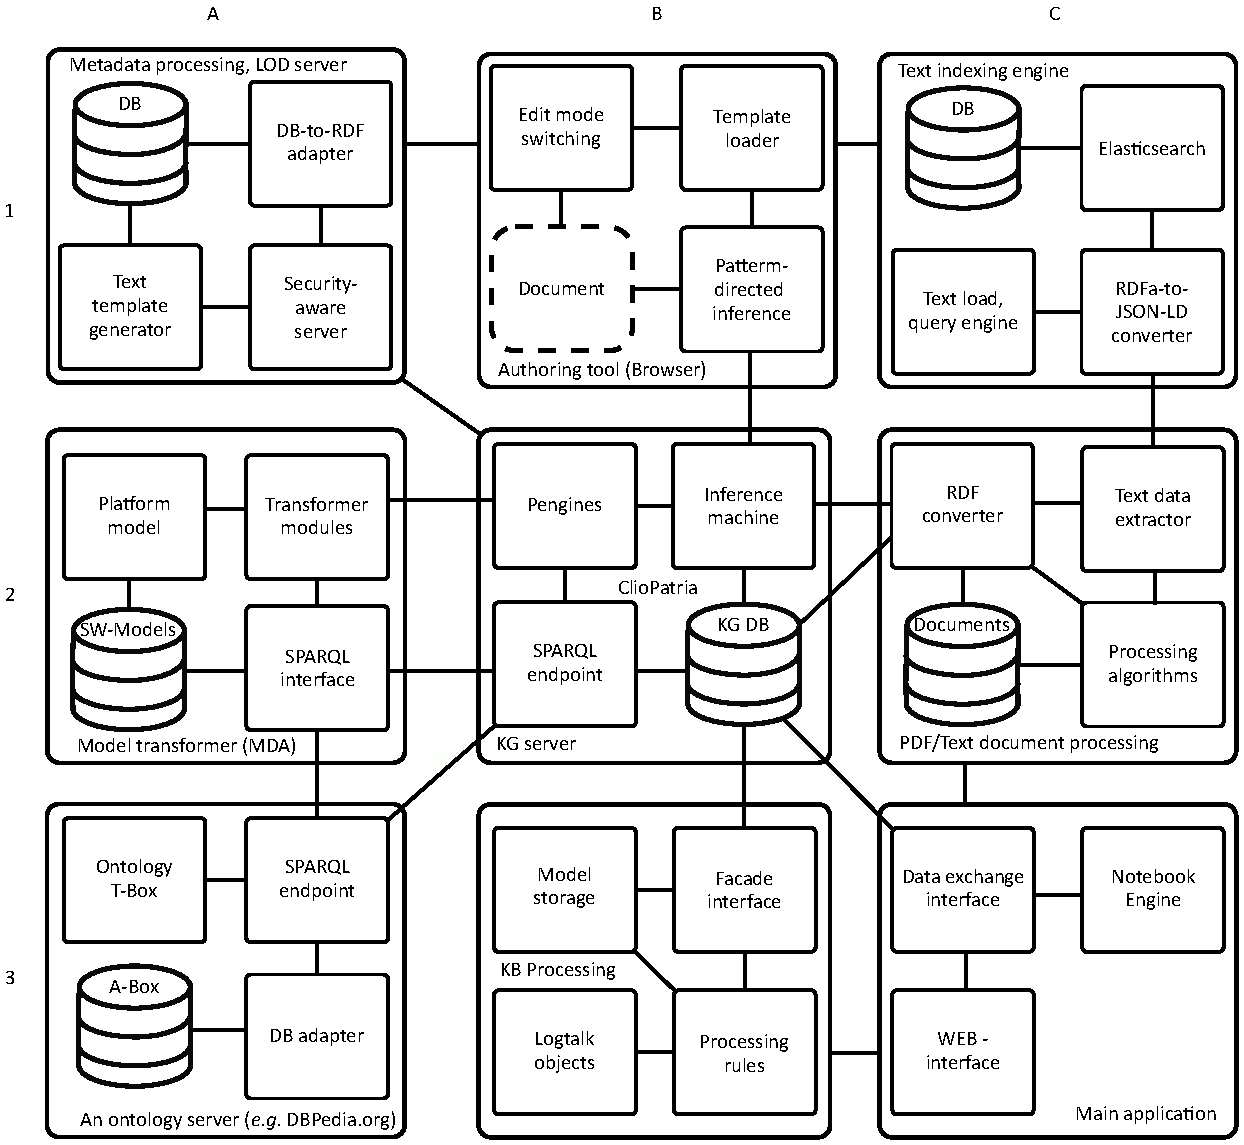
\includegraphics[width=1\linewidth]{architecture-mda-lod-ext-general.pdf}
    \end{column}
    \begin{column}{0.3\linewidth}
      \textbf{Abbreviations}\\[1ex]\scriptsize
      T-Module is Transformation module\\
      MDA is Model-Driven Architecture\\
      CIM is Computationally Independent Model\\
      PIM is Platform Independent Model\\
      PSM is Platform Specific Model\\
      T-Box is Terminological Box\\
      A-Box is Instance Box\\
      A-Box is Instance Box\\
      NGS is Next-Generation Sequencing\\
      DB is Database
    \end{column}
  \end{columns}
\end{frame}

\begin{frame}
  \frametitle{Architecture of transformation modules}
  \centering
  \includegraphics[width=0.9\linewidth]{architect_tree_pres-en-wo-OCL.pdf}
\end{frame}

\begin{frame}
  \frametitle{Logtalk as transformation definition language}
  We have chosen Logtalk as it
  \begin{itemize}
  \item inherits widely known Prolog language syntax and runtime;
  \item implemented as macro package, performance penalties are about 1.5\%;
  \item has flexible semantics: we can define transformations and constraints within the same syntax;
  \item implement object-oriented knowledge (rules) structuring, encapsulation and replacement;
  \item compositional way of transformation implementation;
  \item powerful engine to post constraints on object-to-object messages (events);
  \item has implementation for many Prolog engines.
  \end{itemize}
  The <<regular>> language allow us to use its libraries not directly related to MDA transformations.
\end{frame}

\begin{frame}[fragile]
  \frametitle{RDF (TTL) representation and and its query object}
  \begin{columns}
    \begin{column}{0.4\linewidth}
\begin{minted}[fontsize=\tiny]{turtle}
@prefix xml: <http://www.w3.org/XML/1998/namespace> .
@prefix xsd: <http://www.w3.org/2001/XMLSchema#> .
ngsp:spec a ngsp:Specification ;
    ngsp:module mothur:NoCommand,
        mothur:align-check,
        mothur:align-seqs,
# . . . . .
mothur:align-check a ngsp:Module ;
    ngsp:outputPattern [ a cnt:Chars ;
            ngsp:parameterName "type" ;
            ngsp:pattern [ ngsp:patternString
                    "[filename],align.check" ;
                    dc:identifier "aligncheck" ] ;
            cnt:chars # . . . .
# . . . . .
mothur:align-check-idir-parameter a ngsp:Parameter ;
    ngsp:important false ;
    ngsp:multipleSelectionAllowed false ;
    ngsp:optionsDefault "" ;
    ngsp:required false ;
    ngsp:type mothur:String ;
    dc:title "inputdir" .

mothur:align-check-map-parameter a ngsp:Parameter ;
    ngsp:important true ;
    ngsp:multipleSelectionAllowed false ;
    ngsp:optionsDefault "" ;
    ngsp:required true ;
    ngsp:type mothur:InputTypes ;
    dc:title "map" .

mothur:align-check-name-parameter a ngsp:Parameter ;
    ngsp:chooseOnlyOneGroup "namecount" ;
    ngsp:important false ;
    ngsp:multipleSelectionAllowed false ;
# . . . . .
\end{minted}
    \end{column}
    \begin{column}{0.6\linewidth}
\begin{minted}[fontsize=\scriptsize]{logtalk}
:- object(query(_XMI)).
:- protected(xmi/1).
:- public([class/2, attribute/3, method/3]).
xmi(XMI) :- parameter(1, XMI).
    % Recognition of Class in RDF
class(Name, ID):-
    ::xmi(XMI),
    XMI::rdf(ID,rdf:type,uml:'Class'),
    XMI::rdf(ID,rdfs:label, literal(Name)).
    % Recognition of an attribute
attribute(Name, ClassID, ID):-
    ::xmi(XMI),
    XMI::rdf(ClassID, xmi:ownedAttribute, ID),
    XMI::rdf(ID, rdfs:label, literal(Name)).
    % Recognition of a method specification.
method(Name, ClassID, ID):-
    ::XMI(XMI),
    XMI::rdf(ClassID, xmi:ownedOperation, ID),
    XMI::rdf(ID, rdfs:label, literal(Name)).
% . . . . . . . . . . .
:- end_object.
\end{minted}
    \end{column}
  \end{columns}
\end{frame}

\begin{frame}[fragile]
  \frametitle{Code Block (idea is taken from \texttt{llvmlite}${}^*$)}
  \begin{columns}
    \begin{column}{0.6\textwidth}
      \flushleft
\begin{minted}[fontsize=\footnotesize{}]{logtalk}
:- object(code_block, specializes(root)).
% Public interface of the object
:- public([append/1, prepend/1, clear/0,
   render/1, render_to/1, remove/1,
   item/1, items/1]).
% Code block items
:- dynamic([item_/1]).
:- private([item_/1]).
% Methods specialized during inheritance
:- protected([renderitem/2, render_to/2]).
% . . . . . . . . . . . .
% Delegate rendering to object itself
renderitem(Object, String):-
    current_object(Object), !,
    Object::render(String).
% Convert a literal to its string
% representation
renderitem(literal(Item), String):-!,
    atom_string(Item, String).
% Just print the item (debugging).
renderitem(Item, String):-
    root::iswritef(String, '%q', [Item]).
:- end_object.
\end{minted}
    \end{column}
    \begin{column}{0.4\textwidth}
      \includegraphics[width=1\linewidth]{code_block.pdf}
  ${}^*$) \url{https://github.com/numba/llvmlite}
    \end{column}
  \end{columns}
\end{frame}

\begin{frame}[fragile]
  \frametitle{PSM of a Python Class as a specialization of Code Block}
%\begin{multicols}{2}
  \begin{columns}
    \begin{column}{0.6\textwidth}
      \flushleft
\begin{minted}[fontsize=\scriptsize]{logtalk}
:- object(class, specializes(code_block),
   imports([named])). % Category of named entities
:- public([classlist/1, methods/1, attributes/1]).
% . . . . . . . . . . . . . .
renderitem(Item, Result):-      % proceed with default
    ^^renderitem(Item, Result). % rendering
render(Result):-         % Source generator
    ^^render(Name),      % implemented in a category
    ( ::item(classlist(List)) ->
     % . . . . . . . . . . .
        [Name]) ),
    ( ::item(attributes(Attributes))->
     % . . . . . . . . . . .
        [DefAttrList]),
      Attributes::items(InstanceAttrs),
      findall(S, ( % initialize attributes
         % . . . . . . . . .
         ), AttrAssigns),
        root::unindent,
        AttrList=[ConstructorDef|AttrAssigns];
         % . . . . . . . . .
        AttrList=[ConstructorDef, Pass] ),
    ( ::item(methods(Methods))-> % If any ...
      Methods::render(MethodList);
      MethodList=[] ),
    lists::append(AttrList,MethodList,StringList),
    root::unindent, Result=[Signature|StringList].
:- end_object.
\end{minted}
    \end{column}
    \begin{column}{0.4\linewidth}
      \includegraphics[width=1\linewidth]{code_block_class.pdf}
    \end{column}
  \end{columns}
  % \end{multicols}
\end{frame}

\begin{frame}[fragile]
  \frametitle{Logtalk Categories}
  A category of named entities
\begin{minted}[fontsize=\scriptsize]{logtalk}
:- category(named).
:- public([name/1, render/1]).
:- protected([renderitem/2]).
name(Name):- ::prepend(name(Name)).
renderitem(name(Name), String):-!, atom_string(Name, String).
render(String):-  % What is code generation from items
    ::item(name(Name)), ::renderitem(name(Name), String).
:-end_category.
\end{minted}
Category of named and typed entities
\begin{minted}[fontsize=\scriptsize]{logtalk}
:- category(namedtyped, extends(named)).
:- public([type/1,render/2, separator_option/2,list_separator/1]).
:- protected([renderitem/2]).
type(Type):- ::append(type(Type)).
renderitem(Item, String):- ^^renderitem(Item, String),!.
renderitem(type(Type),String):-!, ::list_separator(Separator),
    writef::swritef(String, '%w%w', [Separator, Type]).
render(Middle, String):- ^^render(SName),
    (   ::item(type(Type)) ->
        ::renderitem(type(Type), SType),
        string_concat(SName, Middle, _1),
        string_concat(_1, SType, String) ;
        SName = String  ).
render(String):-  ::render("", String).
list_separator(Separator):-
    ::separator_option(Name, Default),!, % Global options
    root::option(Name, Separator, Default).
:- end_category.

\end{minted}
\end{frame}

% \begin{frame}
%   \frametitle{Future activities}
%   The future activities supposed to be as follows:
%   \begin{enumerate}
%   \item Having dataflow models of MiSeq SOP and other techniques, device an intelligent subsystem, which will construct computational procedures for a predefined set of data processing tasks (\emph{AI's problem solving}).
%   \item Integrate dataflow and data storage with Galaxy.
%     \begin{itemize}
%        \item Realize adapters of data/metadata storage and retrieving, as well as the storage.
%        \item Create a more sophisticated source code parser or PIM model of computation so we will able to infer metadata for the output on the metadata of input (partially done in November).
%          % \item Adapt our ``pattern-directed'' approach of semantically marked up document authoring to present input and output to the scientific communities.
%        \item Adapt our document authoring tools to Galaxy allowing LOD representation of results.
%   \end{itemize}
%   \item Implement integration to biological/gene databases.
%   \item Write a handbook on Logtalk programming strategies with its author Paulo Mora.
%   \end{enumerate}
% \end{frame}


% \begin{frame}
%   \frametitle{Conclusion}
%   The following results have been obtained as for today:
%   \begin{itemize}
%   \item Biologists' activities are mastered, investigated and regular patterns are described.
%   \item A technique for interpretation of Mothur interfaces has been developed, implemented, refined and extended.
%   \item Transformation tools are tested in application areas and no significant technical problems were detected.
%   \item A technique of document authoring is being developed and adapted to the domain.
%   \item Integration with Galaxy project is the primary aim of the future development.
%   \end{itemize}
%   The source codes are available at \url{https://github.com/isu-enterprise/icc.xmitransform}, \url{https://github.com/eugeneai/icc.mothurpim}.

%   This research is supported by Irkutsk scientific center of SB RAS, project No 4.2;
% \end{frame}

\begin{frame}
  \frametitle{Discussion (MDA application)}
  Interesting positive impressions obtained:
  \begin{itemize}
  \item Logtalk and RDF are flexible, sufficiently universal and convenient implementation infrastructures for MDA;
  \item The best implemenation means is Prolog predicate wrapping and Logtalk object encapsulation of rules;
  \item Not all Logtalk properties are investigated: there might be more sophisticated programming techniques developed, \emph{e.g.}, on the base of message watchers.
  \end{itemize}
  Technical problems making the approach somewhat problematic:
  \begin{itemize}
  \item Very simple tasks take too much efforts, \emph{e.g.}, text processing: convert an identifier into the CamelCase;
  \item It takes too long to surf Internet in order to find a vocabulary for a domain, but it is more productive than development new one and classes;
  \item Prolog is not a popular language in MDA, neither Logtalk.
  \end{itemize}
\end{frame}

\begin{frame}
  \frametitle{Application: Document authoring and storage}
  In most cases documents are created as a result of
  \begin{itemize}
  \item creative activity of a person with a text processors (authoring);
  \item printing a digital copy or a data record in a database;
  \item aggregation operation over database records (report).
  \end{itemize}
  Then it is stored either as a physical paper and/or a digital document (PDF, DOCX, HTML).

  Since 2000-th, Semantic Web and Linked Open Data (LOD) is being developed, allowing
  \begin{itemize}
  \item structural storage of data within published documents;
  \item processing stored data computationally;
  \item integration of data structures and data objects globally.
  \end{itemize}

  The \textbf{aim of this research} is to develop technologies, software and services allowing construction of digital archives supporting document data inclusion and inference from existing documents.
\end{frame}

\begin{frame}
  \frametitle{Structure of a document}
  \centering
  \includegraphics[width=1\linewidth]{document-structural-view.pdf}
\end{frame}

\begin{frame}
  \frametitle{Open Annotation (oa)}
\begin{adjustwidth}{-3em}{-3em}
  \centering
 \includegraphics[width=1\linewidth]{Open-Annotation_CB_Bookmarking_and_Semantically_Tagging_A_webpage_spec20130128.png}
\end{adjustwidth}
\end{frame}


\begin{frame}
  \frametitle{Architecture}
  \begin{adjustwidth}{-2.5em}{-2.5em}
    \begin{center}
      \includegraphics[width=0.5\linewidth]{architecture-mda-lod-ext-tot.pdf}
    \end{center}
  \end{adjustwidth}

% \begin{itemize}
% \item content and metadata repository with SPARQL (6) and full-text search (3); the engines for LOD processing (5) based on the logical inference;
% \item service for analysis of the stored content (2) enriching the archive with semantic information describing the content;
% \item tools for development of LOD applications and their user interfaces (1);
% \item browser based authoring tools (4).
% \end{itemize}
\end{frame}

\begin{frame}
  \frametitle{Generated list of title page preambles}
    \begin{adjustwidth}{-2.5em}{-2.5em}
    \begin{center}
      \includegraphics[width=0.7\linewidth]{template-title-pages.jpg}
    \end{center}
  \end{adjustwidth}
\end{frame}

\begin{frame}
  \frametitle{Generated part of a study program}
   \begin{adjustwidth}{-2.5em}{-2.5em}
    \begin{center}
      \includegraphics[width=0.7\linewidth]{template-courses.jpg}
    \end{center}
  \end{adjustwidth}
\end{frame}
\begin{frame}
  \frametitle{Imported time distribution for lecture, seminary, \ldots}
   \begin{adjustwidth}{-2.5em}{-2.5em}
    \begin{center}
      \includegraphics[width=0.9\linewidth]{work-program-volume.jpg}
    \end{center}
  \end{adjustwidth}
\end{frame}


\begin{frame}[fragile]
  \frametitle{Representation of  document parts with RDFa}
  % \begin{block}{}
  %   \textbf{Целью} исследования является создание методики разработки процедур трансформации (PD\footnote{Platform [description] model.}) в виде ОО-модулей.
  % \end{block}
  % \begin{columns}
  %   \begin{column}{0.5\linewidth}
  %     % \includegraphics[width=1\linewidth]{pics/scenario-ru-wo-mothur.pdf}
  %   \end{column}
  %   \begin{column}{0.6\linewidth}
  %     Задачи исследования:
  %     \begin{itemize}
  %     \item Изучить синтаксические структуры Logtalk в аспекте структурирования знаний;
  %     \item Предложить методику представления трансформации в виде ОО-модулей;
  %     \item Реализовать библиотеку объектов и классов для МДА;
  %     \item Тестирование библиотеки на примере.
  %     \end{itemize}
  %   \end{column}
  % \end{columns}

\begin{adjustwidth}{-1.5em}{-1.5em}
\begin{minted}[escapeinside=||,fontsize=\btprgsize]{text}
<html lang="ru" xmlns=http://www.w3.org/1999/xhtml
|\GB{xmlns:taa}|=http://irnok.net/engine/rdfa-manipulation
xml:lang="ru" metal:define-macro="page">
<head> . . . . </head>
<body prefix="rdf: http://www.w3.org/1999/...-ns# foaf: http://xmlns.com/foaf/...
imei: imei.html# course: https://irnok.net/college/plan/01..16-...\
%D0\%BA_PB-SM.plm.xml.xlsx-....2.3.1.html#"  resource="#post"
typeof="schema:CreativeWork sioc:Post prov:Entity">
<!-- The application control panel -->

<main lang="ru" resource="#annotation" typeof="oa:Annotation" id="main-doc-cnt">
<div property="oa:hasTarget" resource="#course-work-prog"></div>
<article property="oa:hasBody" typeof="foaf:Document curr:WorkingProgram"
         resource="#course-work-program" id="main-document">
  <div |\GB{taa:content}|="imei:title-page"></div>
  <div |\GB{taa:content}|="imei:neg-UMK"></div>
  <section id="TOC" class="break-after"> <h2>Table of Contents</h2>
    <div id="tableOfContents"></div>
  </section>
  <section id="course-description" resource="#description"
           property="schema:hasPart" typeof="schema:CreativeWork">
    <div property="schema:hasPart" resource="#purpose"
         typeof="dc:Text cnt:ContentAsText" >
      <div property="cnt:chars" datatype="xsd:string">
        <h2 property="dc:title" datatype="xsd:string">
           Aims and objectives of the discipline (module)</h2>
        <p>The aim of teaching the discipline ...</p>
      </div>
   </div>
  . . . . . . . .
\end{minted}
\end{adjustwidth}
\end{frame}


\begin{frame}
  \frametitle{Complete document}
  \begin{adjustwidth}{-2.5em}{-2.5em}
    \begin{center}
      \begin{columns}
        \begin{column}{0.5\linewidth}
          \includegraphics[width=1\linewidth]{work-program-title.jpg}
        \end{column}
        \begin{column}{0.5\linewidth}
          \includegraphics[width=1\linewidth]{work-program-agreement.jpg}
        \end{column}
    \end{columns}
    \end{center}
  \end{adjustwidth}
\end{frame}

\begin{frame}
  \frametitle{Discussion}
A tools (components) for digital archive implementation, which allows
to device information systems and document processing services
with the following features:
\begin{itemize}
\item load LOD marked up document, extract, store in a graph and index RDF data;
\item retrieve RDF data as triples or as a result of full-text search query;
\item combine existing LOD data and its content in new documents dynamically with browser based context inference machine;
\item use server-site inference machine (Prolog) to process RDF data upon
  request from browser's part of the system;
  % \item organizes a platform for document semantic markup,
\item convert created RDFa marked up HTML5 documents into Excel and Word formats.
\end{itemize}

  \textbf{Applications}
  \begin{itemize}
  \item Document authoring automation;
  \item Context-depended editing;
  % \item Export into office formats;
  \item Self-organizing global document flows;
  \item Documents as data sources for information systems.
  \end{itemize}

\end{frame}

\begin{frame}
\frametitle{Application: Cartographical WEB-service with knowledge graph of South-Siberian faults}
\textbf{Aim} is to construct a WEB-GIS browser for faults stored in the KG.
\begin{itemize}
\item Scalability to external data with converters (TODO)
\item Interdisciplinary data representation
\item Application development with nowadays WEB techniques
\item Digital platform for data publication in ``Digital Baikal'' project
\end{itemize}
% \end{frame}

% \begin{frame}
% \frametitle{Key points}
Development \textbf{plan}
\begin{itemize}
\item Investigate the current data formats
\item Develop T-Box
\item Fill in A-Box
\item Expose the KG with a server
\item Implement browsing SPARQL query results with GIS
\item Develop object browser
\end{itemize}
MVP is a WEB-GIS with the most of the listed features.
\end{frame}

\begin{frame}
  \frametitle{GIS source data table properties}
  \begin{itemize}
  \item Only one table, one row for each GIS object
  \item There are many \texttt{NULL} values
  \item More than 1000 objects
  \item More than 70 attributes (according to O.V.~Lunina, PhD)
  \end{itemize}
  \begin{center}
    \includegraphics[width=1\linewidth]{gis-fault-table.png}
  \end{center}
\end{frame}


\begin{frame}
\frametitle{Developed ontology}
The ontology contains nonintersection properties for its classes
\begin{center}
    \includegraphics[width=1\linewidth]{fault-onto.png}
\end{center}
\end{frame}

\begin{frame}
\frametitle{Serving ontology and its A-box}
As server \texttt{GraphDB} is used.
\begin{center}
    \includegraphics[width=1\linewidth]{graph-db.png}
\end{center}
\end{frame}

\begin{frame}
\frametitle{Web GIS}
\begin{center}
    \includegraphics[width=1\linewidth]{gis-ex.png}
\end{center}
\end{frame}

\begin{frame}
\frametitle{Used technologies for constructing WEB-GIS browser}
\begin{center}
    \includegraphics[width=1\linewidth]{gis-tech.png}
\end{center}
\end{frame}

\begin{frame}[fragile]
  \frametitle{Ontological instruments: editor Proteg\'e}
  \begin{columns}
    \begin{column}{0.4\textwidth}
      \includegraphics[width=1\linewidth]{pics/NLP-fault-tbox-shot.png}
    \end{column}
    \begin{column}{0.6\textwidth}
      \includegraphics[width=1\linewidth]{pics/NLP-fault-abox-shot.png}
    \end{column}
  \end{columns}
\end{frame}

\begin{frame}[fragile]
  \frametitle{Modification of GeoBase supporting Semantic WEB}
\begin{minted}{prolog}
schema('fault','in','continent').  % Connect our relations with GeoBase
schema('fault','with','feature').  % vocabulary.
schema('name','of','fault').       %
% schema('feature','of','fault').  % This relation is already in the T-Box''

% Interpret any well described relation
% between a subject (fault) via ''of''.
schema(Prop, 'of', SubjName):-     % used on translation stage
        var(SubjName),
        geob_prop(Prop,_).

schema(Prop, 'of', SubjName):-     % used on stage of interpretation
        nonvar(SubjName),          % a Class is supplied
        geob_prop(Prop, GProp),
        geob_ent_class(SubjName, Subj),
        rdf_reachable(Subj, rdfs:subClassOf, Parent),
        rdf(GProp, rdfs:domain, Parent),!.

geob_prop(Prop, GProp):-           % Property check
        rdf_global_id(geob:Prop, GProp),
        rdf(GProp,rdf:type,owl:'ObjectProperty'),!.

geob_class(Class, GClass):-        % Class check
        rdf_global_id(geob:Class, GClass),
        rdf(GClass,rdf:type,owl:'Class'),!.

geob_ent_class(Ent, Class):-
        sub_atom(Ent,0,1,R,H),
        sub_atom(Ent,1,R,0,T),
        string_upper(H,U),
        atom_concat(U,T,GEnt),
        geob_class(GEnt, Class).

geob_ent(E, A):-
        nonvar(E),
        geob_ent_class(E,Class),
        rdf(A, rdf:type, Class, geodata). % A Subject of geodata
\end{minted}
\end{frame}

\begin{frame}[fragile]
  \frametitle{GeoBase to ActiveFaults Natural language interface}
  \begin{center}
    \includegraphics[width=1\linewidth]{Geobase-ui.png}
  \end{center}
  \textbf{New problem} for student graduation project: Implement Natural Language to SPARQL translator.
\end{frame}

% \begin{frame}
%   \frametitle{Conclusion}  % On Web GIS
%   The following results have been obtained as for today:
%   \begin{itemize}
%   \item A technique for \textbf{domain} model representation has been developed and tested.
%   \item A programming technique using object-oriented logical language Logtalk is devised.
%   \item Prototypes of various transformation procedures are implemented.
%   \item Transformation tools are tested in application areas and no significant technical problems were mentioned.
%   \end{itemize}
%   Further development directions are as follows:
%   \begin{itemize}
%   \item A technique for document automatic markup with vocabulary entities.
%   \item A transformation implemenation techniques, minimizing usage of dynamic objects, targeting on macro properties of Logtalk.
%   \item Form a toolset out of existing prototypes obeying nowadays software development requirements.
%   \end{itemize}
%   Projects sources are at \url{https://github.com/isu-enterprise} and \url{https://github.com/eugeneai}.
% \end{frame}

\begin{frame}
  \frametitle{Conclusion}  % On Web GIS
  Web-3.0 (SW and KG) are convenient and productive basis of application development, allowing one to
  \begin{itemize}
  \item Integrate on various levels of software representation, \emph{i.e.}, from data to abstract models.
  \item There are assets to utilize global resources in applications (\texttt{DBPedia.org}).
  \item The inherited software are involved via adapters.
  \end{itemize}
  In our projects we has been developed techniques to
  \begin{itemize}
  \item Data processing and model transformation using Prolog-based logical inference.
  \item Logtalk is a perfect instrument for knowledge encapsulation and processing, complex data synthesis.
  \end{itemize}
\end{frame}

% \begin{frame}
%   \frametitle{Technologies used (open source)}
%   Python-3.x.x (\url{http://python.org}),\\
%   ZCA (\url{https://muthukadan.net/docs/zca.html}),\\
%   SWIG (\url{http://swig.org/}),\\
%   SWI-Prolog (\url{https://www.swi-prolog.org/}),\\
%   Logtalk (\url{https://logtalk.org/}),\\
%   ClioPatria (\url{https://cliopatria.swi-prolog.org/home}),\\
%   Pengines (\url{https://pengines.swi-prolog.org/docs/index.html}),\\
%   LOV (\url{https://lov.linkeddata.es/dataset/lov/}),\\
%   Elastic Search (\url{https://www.elastic.co/}),\\
%   Kyotocabinet (\url{https://fallabs.com/kyotocabinet/}),\\
%   DBPedia (\url{https://wiki.dbpedia.org/}),\\
%   Mothur (\url{https://mothur.org/}),\\
%   Galaxy (\url{https://usegalaxy.org/}),\\
%   R (\url{https://www.r-project.org/}), \\
%   Dust.js (\url{https://akdubya.github.io/dustjs/})
% \end{frame}

\begin{frame}
  \begin{center}
  \Large Thanks for Your Attention!
\end{center}
\end{frame}



\end{document}

%%% Local Variables:
%%% mode: latex
%%% TeX-master: t
%%% End:
